\documentclass[./main.tex]{subfiles}

\begin{document}
\begin{figure}[htbp]
    \centering
    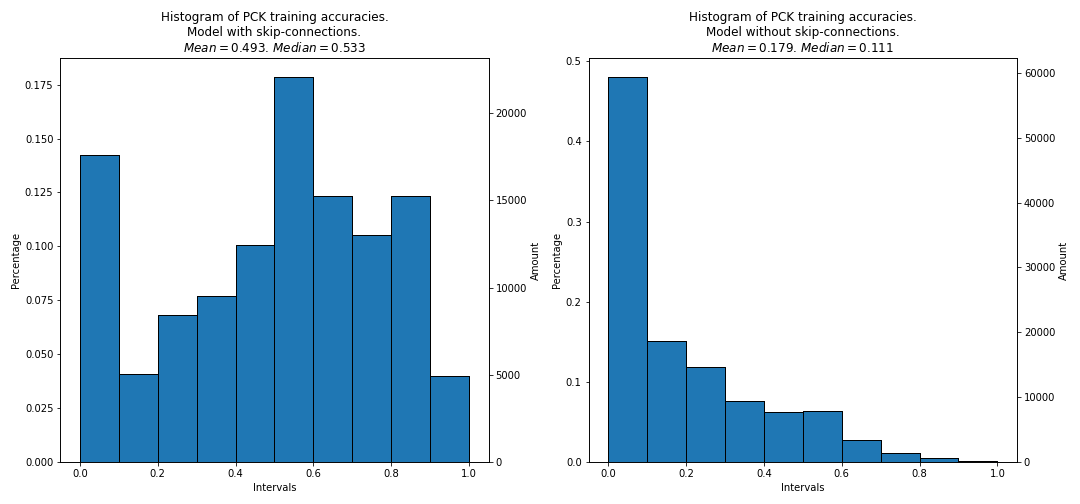
\includegraphics[height = 6 cm]{entities/PCK_accs_vs.png}
    \caption{Histogram of PCK training accuracies of the model with the skip-connections enabled (left) and the model with the skip connections disabled (right).}
    \label{fig:PCK_accs}
\end{figure}

\section{Interpreting the Model}\label{sec:XAI}
In the following section we will be interpreting the model developed in section \ref{experiement}, with the intention of getting an understanding of what the model has learned during training, what the different parts of the model are used for, as well as checking for any redundancy in the model. In Section \ref{subsec:motivation_xai} an overview of the motivation behind interpreting the model is given. Section \ref{subsec:verifying_skip_cons} then evaluates the effects of the skip-connections of the model. Then, Section \ref{subsec:shape_analysis} explores the latent space of the model with respect to getting an understanding of the principal components of the latent space. Section \ref{subsec:clustering} also explores the latent space of the model, however, instead it uses clustering to seperate the latent space, which the results are the discussed.

\subsection{Motivation}\label{subsec:motivation_xai}
Deep learning models are often complex and work like a \textit{black boxes}. By that it is meant, that when a network is given some input, the model simply just returns some output without any explanation or reasoning behind the output. This can often be a problem, especially in cases where the output of the network can result in a life or death situation of a human. For that reason, understanding and explaining how a network works can be very important - this is what is called \textit{explainable AI} (\textit{XAI}) 
\\
\\
Selvaraju \textit{et al.} \cite{Selvaraju} argues that there are three cases for using explainable AI:
\begin{enumerate}
    \item When the network performs worse than humans, an understanding of the network can help us improve the performance of the model.
    \item When the network is on par with humans, an understanding of the network is trivial for humans to build trust in the network, as we can understand its strengths and weaknesses
    \item When the network performs better than humans, an understanding of the network can teach humans how to perform better.
\end{enumerate}
Throughout section \ref{sec:XAI} we will be exploring and understanding what the model, developed in section \ref{experiement}, learned during training and what the different parts of the model are used for, leading towards improving the performance of the model easier.
% MÅSKE OGSÅ, AT VI VIL FORBEDRE MODELLEN!

\subsection{Verifying the Effects of Skip-Connections}\label{subsec:verifying_skip_cons}
Olsen \cite{Camilla} and Newell \cite{Newell} claims, that the skip-connections are used in order to recreate details that are lost during the encoder-phase. Throughout subsection \ref{subsec:verifying_skip_cons} we will be verifying or refuting the claim of the effect of the skip-connections. To do so we will be using two models based on the same network:
\begin{enumerate}
    \item The trained Stacked Hourglass from section \ref{experiement}
    \item The trained Stacked Hourglass from section \ref{experiement}, but with the skip-connections disabled.
\end{enumerate}
Thus, the second model has not been retrained and is identical to the first model, however, without its skip-connections.
\\
\\
In Figure \ref{fig:PCK_accs} the distributions of the PCK training accuracies of the two models have been visualized. We have decided to make use of the training data for computing the PCK accuracies, as we want to look at the data, that the model has been trained on. By looking at the two distributions we can clearly see how to model without its skip-connections performs much worse, than the model with its skip-connections.
\\
\\
To further understand the decrease of accuracy in the case where the skip-connections are disabled, we have in Figure \ref{fig:pred_comparison} visualized $20$ samples from the training dataset, where the model with skip-connections has an $100\%$ PCK accuracy score. Next to each image the ground truth heatmaps, or the prediction by the model with skip-connections, and the prediction by the model without skip-connections has been visualized.
\\
\begin{figure}[htbp]
    \centering
    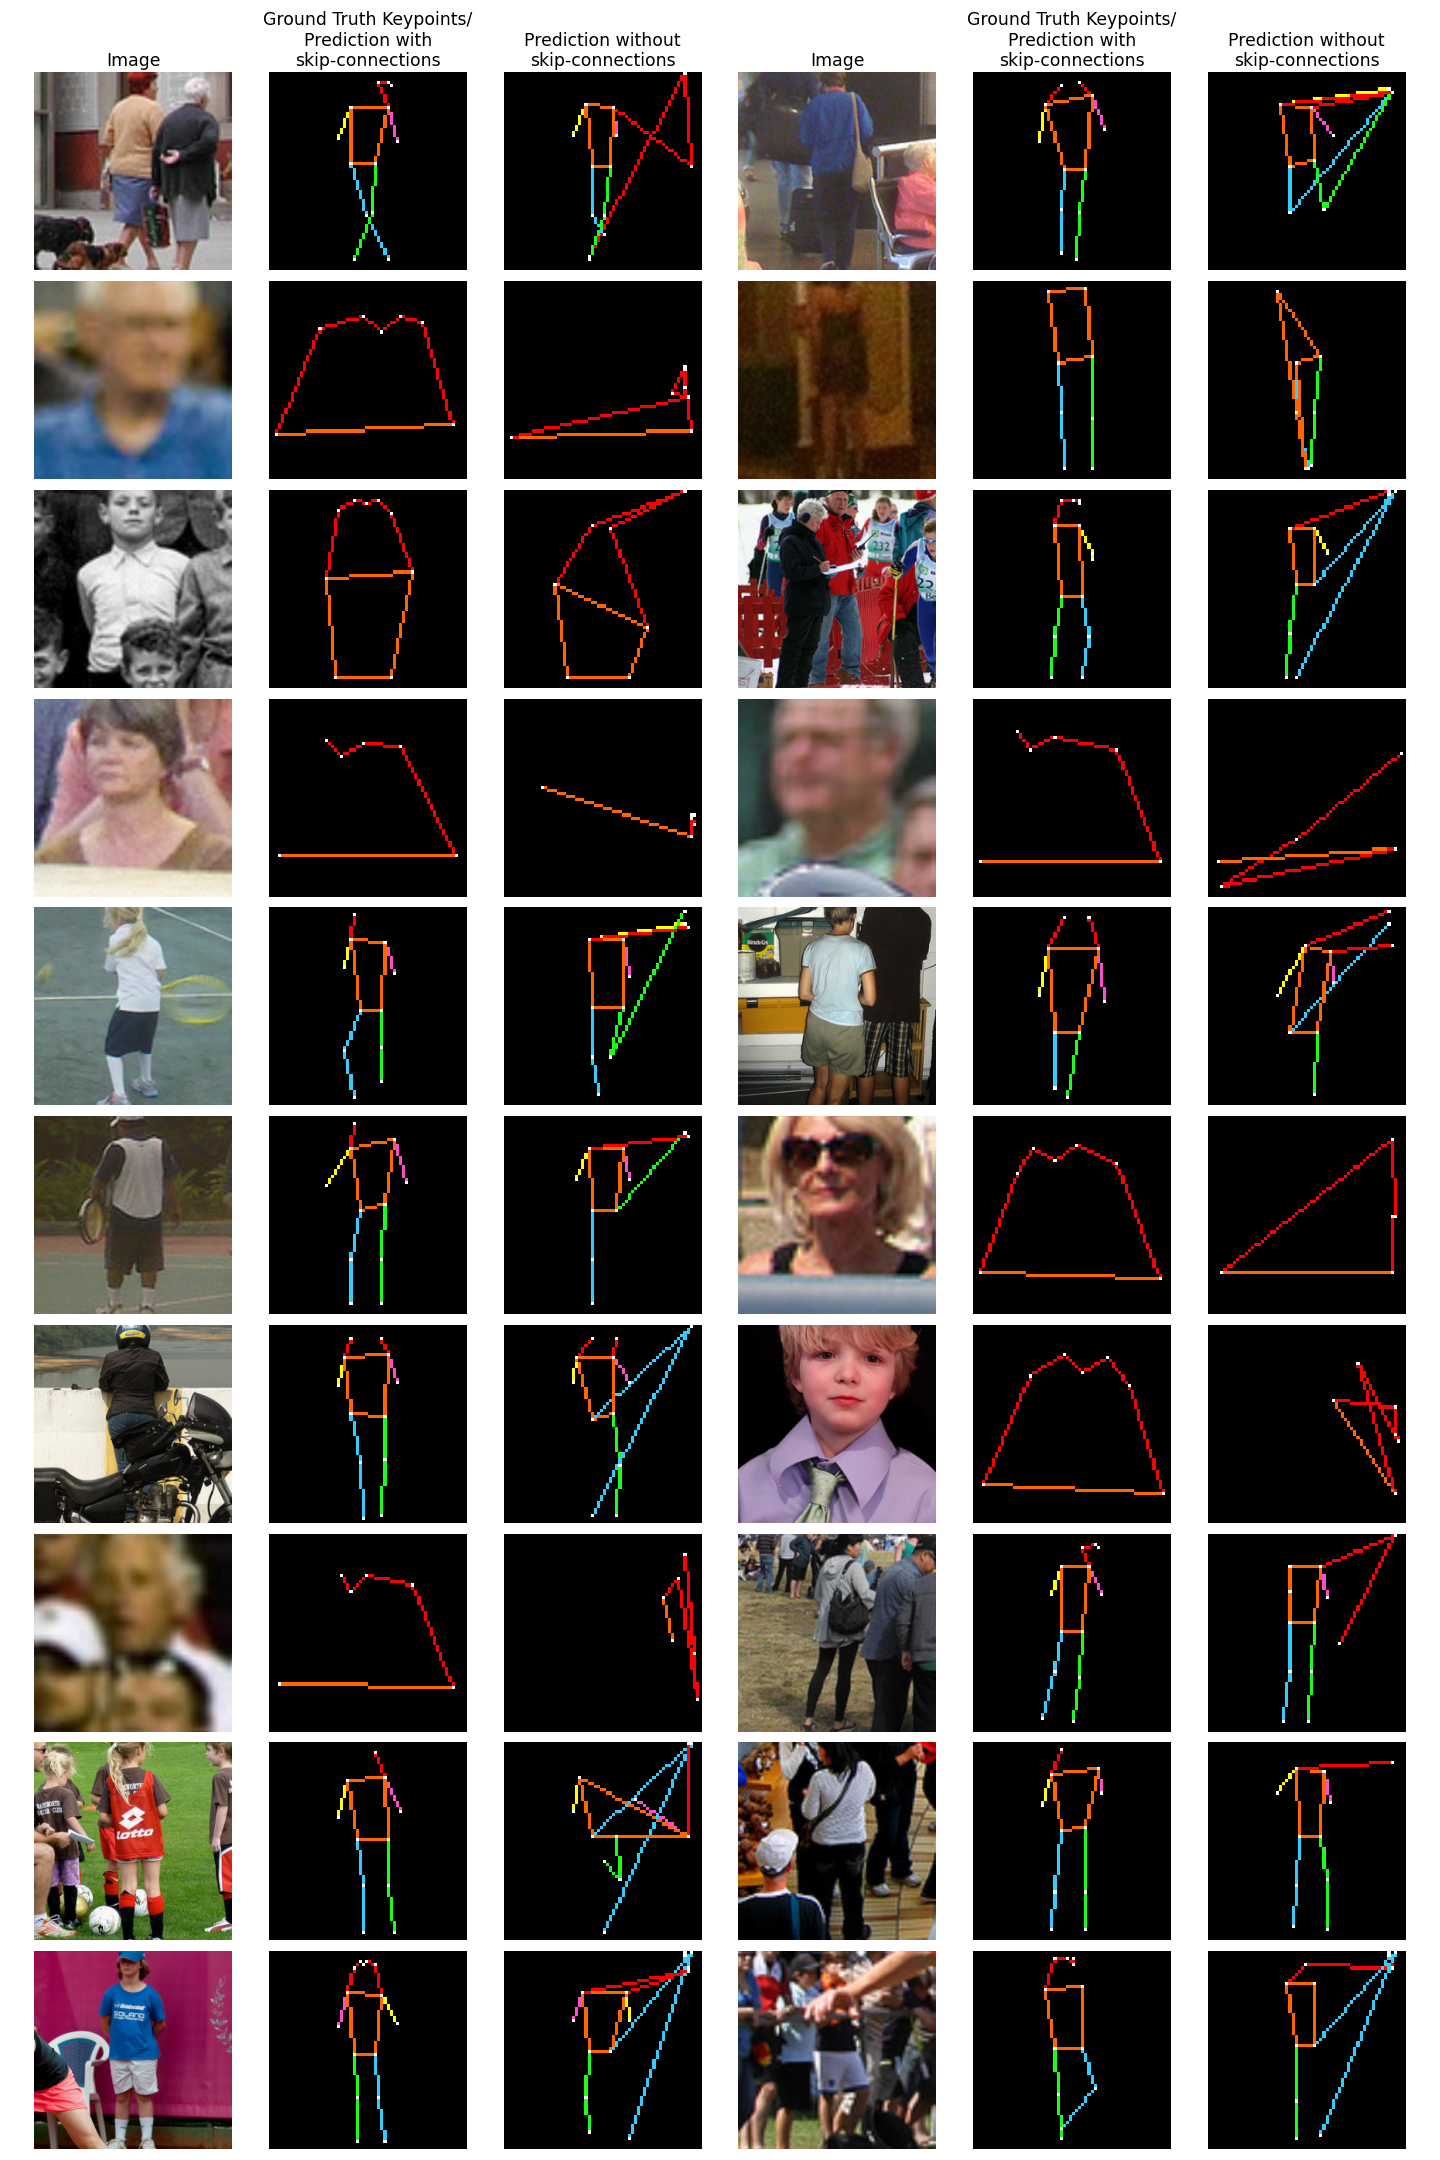
\includegraphics[width = \textwidth]{entities/pred_comparisons.png}
    \caption{20 samples of images correctly predicted by the model with skip-connections enabled, the corresponding ground truth heatmap and predictions by the model with skip-connections disabled.}
    \label{fig:pred_comparison}
\end{figure}
\\
By looking at Figure \ref{fig:pred_comparison} we can see, that the model without its skip-connections often struggles with smaller joints, such as the eyes, ears or nose, whereas it performs better, however still not always perfect, on bigger joints, such as the shoulders, hips or knees. This is probably due to the fact, that the details of the smaller joints has a bigger chance of being lost by the max pooling layers in the encoder. Without the skip-connections their information is thus lost, resulting in bad predictions. Thus, we can verify Olsen's \cite{Camilla} and Newell's \cite{Newell} claims, that the skip-connections are used for recreating details lost in the encoder. 

\subsection{Shape Analysis of the Latent Space}\label{subsec:shape_analysis}
In subsection \ref{subsec:reasoning} we described how we decided to use the Stacked Hourglass for the pose estimation, as it is similar to Autoencoders. This makes the model useful for encoding the data into a lower dimensional representation of the input data. The space of this lower dimensional representation is known as the \textit{latent space} of the model. By exploring the latent space we can get an understanding of what the model has learned during training.
\\
\\
In the following subsection we will be exploring and explaining the most important components of the training data. By doing so we will get an understanding of how each component contributes to a prediction.
\\
\\
We decided to only use fully-annotated observations, as not fully-annotated observations would add some variance to the data, which would confuse the following procedure. We start off by feeding the fully-annotated training data through the encoder of the model and storing the output of the third residual module in the bottleneck. We decided to make use of training data for this, as we wish to look at what features of the training data that the model has learned. Each output of the bottleneck is a $4 \times 4 \times 256$ tensor, which we flattened to a $4.096$ vector. Each vector was then stacked, forming a $7.017 \times 4.096$ matrix of the latent space.
\\
\\
We start off by finding the $4.096$ principal components and the corresponding explained variance ratio of the data by using Principal Components Analysis. By doing so we get an understanding of which components for predictions are the most important. Next, the mean coordinate of the principal components, $\bar{\bm{x}}$ is found. The closest point is then stored. We then explore each principal component by "walking" from $\bar{\bm{x}}$ along the principal component in positive and negative direction, with various step sizes. After each "walk" the closest point is found and stored. By doing so we can compare the heatmaps of the observations from a "walk" in positive and negative direction, which will give us an idea of what a given component is used for. 
\\
\\
When doing the walk along a principal component, we made the step size be equal to $c \cdot \sqrt{\lambda}$, where $c$ is a constant and $\lambda$ is the explained variance of the principal component. By doing so we ensure, that we are not walking too far, ending up with misleading visualizations as there will be far from the end point to the nearest observation. Some of the results have been visualized in Figure \ref{fig:shape_analysis}.
\\
\\
By looking at Figure \ref{fig:shape_analysis} we can see, that the first principal component is used for determining if the person is sitting or standing up. This is very clear, as the person sits down if we are "walking" in the negative direction from the mean coordinate, and on the otherhand the person straightens up if we are "walking" in the positive direction from the mean coordinate.
\\
\\
We can also see, that principal component $2$, $3$, $10$ and $30$ do not have an easy-to-see pattern, like it is the case with the first principal component. This could probably be becuase they explain a very little amount of the variance in the data, resulting in a very small step size, as well as patterns contributing very little to the prediction of the model.
\\
\\
Lastly, we can see, that principal components $50$ and onwards do not have any variations in their corresponding results. This results in them acting as noise, and hints towards how the model could be using many fewer filters in the bottleneck.
\begin{figure}[htbp]
    \centering
    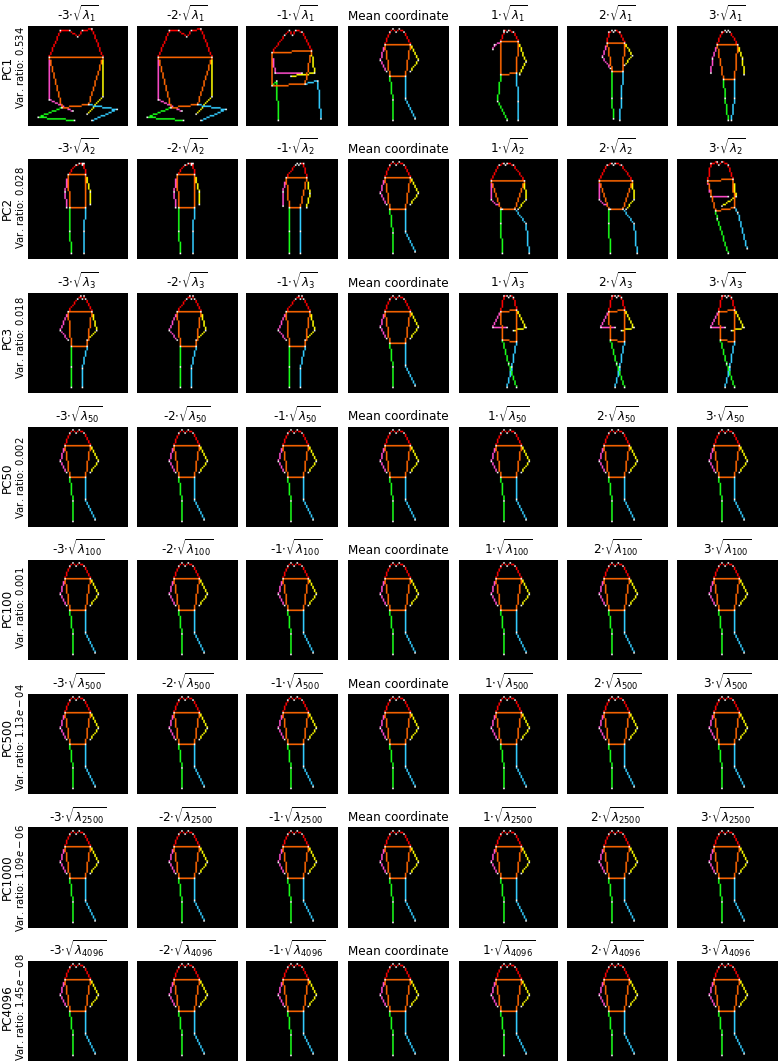
\includegraphics[width = \textwidth]{entities/shape_analysis.png}
    \caption{Nearest observations to the end point of "walking" along various principal components with varying step sizes.}
    \label{fig:shape_analysis}
\end{figure}
\\
\\
All in all, by doing the shape analysis of the latent space of the hourglass, we have learned how the model has learned the difference between people sitting down and standing up (and the poses in between), as well as possibly have identified some redundancy, in the form of the model using more filters in the bottleneck, than what might is needed. 
\begin{figure}[htbp]
    \centering
    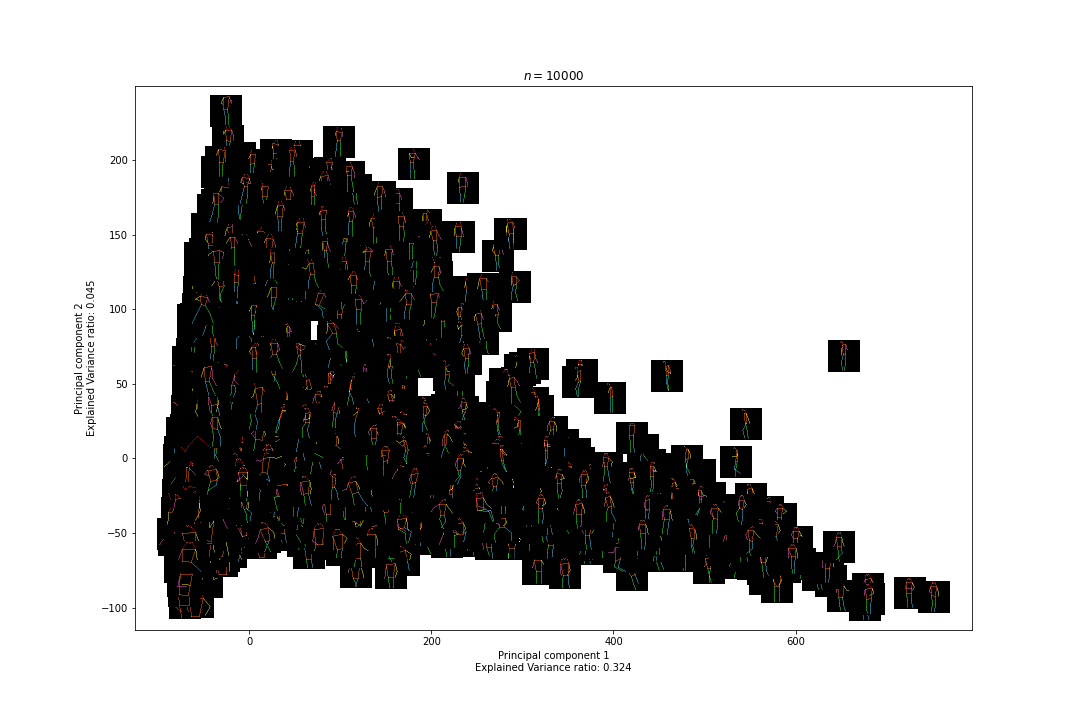
\includegraphics[width = \textwidth]{entities/latent_space_all_skeletons.png}
    \caption{Plot of $10.000$ samples of the latent space of the trained model, with the corresponding ground truth heatmaps}
    \label{fig:latent_space_all_skeletons}
\end{figure}
\subsection{Using Clustering to Seperate the Latent Space}\label{subsec:clustering}
Similar to subsection \ref{subsec:shape_analysis}, we will be exploring the latent space of the model to further get an understanding of what the model has learned during training, where we again will be using the training observations. Instead of exploring the principal components of the latent space, we will instead be grouping the training observations to get an understanding of how the model relate similar data to each other.
\\
\\
To create the latent space matrix we follow the same procedure as in \ref{subsec:shape_analysis}, but instead also use not fully-annotated observations. Due to memory constraints only $10.000$ random samples were used, resulting in an $10.000 \times 4.096$ matrix of the latent space
\\
\\
If we take this latent space matrix, project it down to $2$ dimensions using PCA and visualize the samples with their corresponding ground truth heatmaps, we get the plot visualized in Figure \ref{fig:latent_space_all_skeletons}. The plot only explains about $37\%$ of the variance of the original data, however, we can clearly see how there is some specific structure in the data, as samples that are somewhat similar are close to each other, however, with a few outliers.
\\
\begin{algorithm}[htbp]
    \caption{Compute Silhouette Score \cite{MAD_L12}}
    \label{Algorithm:Silhouette_score}
    \begin{algorithmic}[1]
        \Require Clusters $\bm{C}_0, \bm{C}_1, ..., \bm{C}_{k - 1}$
        \ForAll{cluster $\bm{C}_i$}
            \ForAll{sample $\bm{x} \in \bm{C}_i$}
                \State \begin{varwidth}[t]{\linewidth}
                    Compute the mean euclidean distance from $\bm{x}$ to the other samples in the same cluster: $a(\bm{x}) = \frac{1}{|\bm{C}_i| - 1} \sum_{\bm{y} \in \bm{C}_i} D(\bm{x}, \bm{y})$
                \end{varwidth}
                \State \begin{varwidth}[t]{\linewidth}
                Compute the mean euclidean distance from $\bm{x}$ to the nearest other cluster: $\bm{C}_j$ $b(\bm{x}) = \frac{1}{| \bm{C}_j |} \sum_{\bm{z} \in \bm{C}_j} D(\bm{x}, \bm{z})$
                \end{varwidth}
                \State Compute the Silhouette of $\bm{x}$:
                \begin{math}
                    s(\bm{x}) =
                    \begin{cases}
                        1 - \frac{a(\bm{x})}{b(\bm{x})} & \text{if } a(\bm{x}) < b(\bm{x}) \\
                        0 & \text{if } a(\bm{x}) = b(\bm{x}) \text{ or } |\bm{C}_i| = 1 \\
                        \frac{b(\bm{x})}{a(\bm{x})} - 1 & \text{if } a(\bm{x}) > b(\bm{x})
                    \end{cases}
                \end{math}
            \EndFor
        \EndFor
        \State \textbf{return} mean of the Silhouettes
    \end{algorithmic}
\end{algorithm}
\\
To see how to model seperates the data in the latent space, we will be using $K$-Means. Choosing the optimal $K$ can often be difficult, as it is often not clear how many clusters there are in the data. For choosing the optimal $k$ the \textit{Silhouette score} is often computed, following the pseudocode visualized in Algorithm \ref{Algorithm:Silhouette_score}. For computing the Silhouette score, various values of $K$ are used for training various $K$-Means models. After each model has been trained, let $a_i$ be the average distance of the $i$th sample to the other samples in the same cluster as $i$th sample. Then, let $b_i$ be the average distance of the $i$th sample to the samples in the nearest cluster. Ideally, we want $a_i < b_i$, as $b_i < a_i$ means that the $i$th sample probably has been grouped to the wrong cluster. For that reason, the $i$th silhouette score is set to $1 - \frac{a_i}{b_i}$ if $a_i < b_i$ or $\frac{b_i}{a_i} - 1$ if $a_i > b_i$. By the end of the algorithm the mean silhouette score is returned. By computing the silhouette score for various values of $K$, the $K$ with the silhouette score closest to $1$ is chosen as the optimal $K$ \cite{MAD_L12}.
\\
\begin{figure}[htbp]
    \centering
    \begin{subfigure}{7 cm}
        \centering
        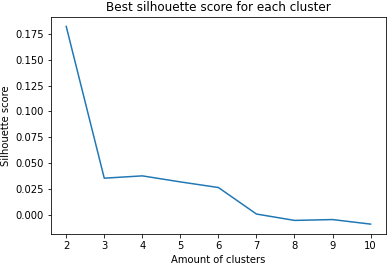
\includegraphics[width = 7 cm]{entities/silhouette_score_all_skeletons.png}
        \caption{Latent space consists of $10.000$ randomly chosen training samples}
        \label{fig:silhouette_all}
    \end{subfigure}
    \begin{subfigure}{7 cm}
        \centering
        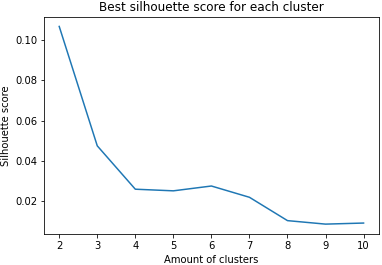
\includegraphics[width = 7 cm]{entities/silhouette_score_full_skeletons.png}
        \caption{Latent space consists of $7.017$ fully-annotated training samples.}
        \label{fig:silhouette_full}
    \end{subfigure}
    \caption{Silhouette score of running various $K$-Means models on different data from the latent space.}
\end{figure}
\\
When running the $K$-Means algorithm on the latent space, we use $K = 2, 3, ..., 10$, where the algorithm is retrained $10$ times with different initial centroid position for each $K$. For each run we record the Silhouette score, where the highest Silhouette score for each $K$ has been visualized in Figure \ref{fig:silhouette_all}. By looking at Figure \ref{fig:silhouette_all} we can clearly see, how the optimal $K$ for the model is when $K = 2$.
\\
\begin{figure}[htbp]
    \centering
    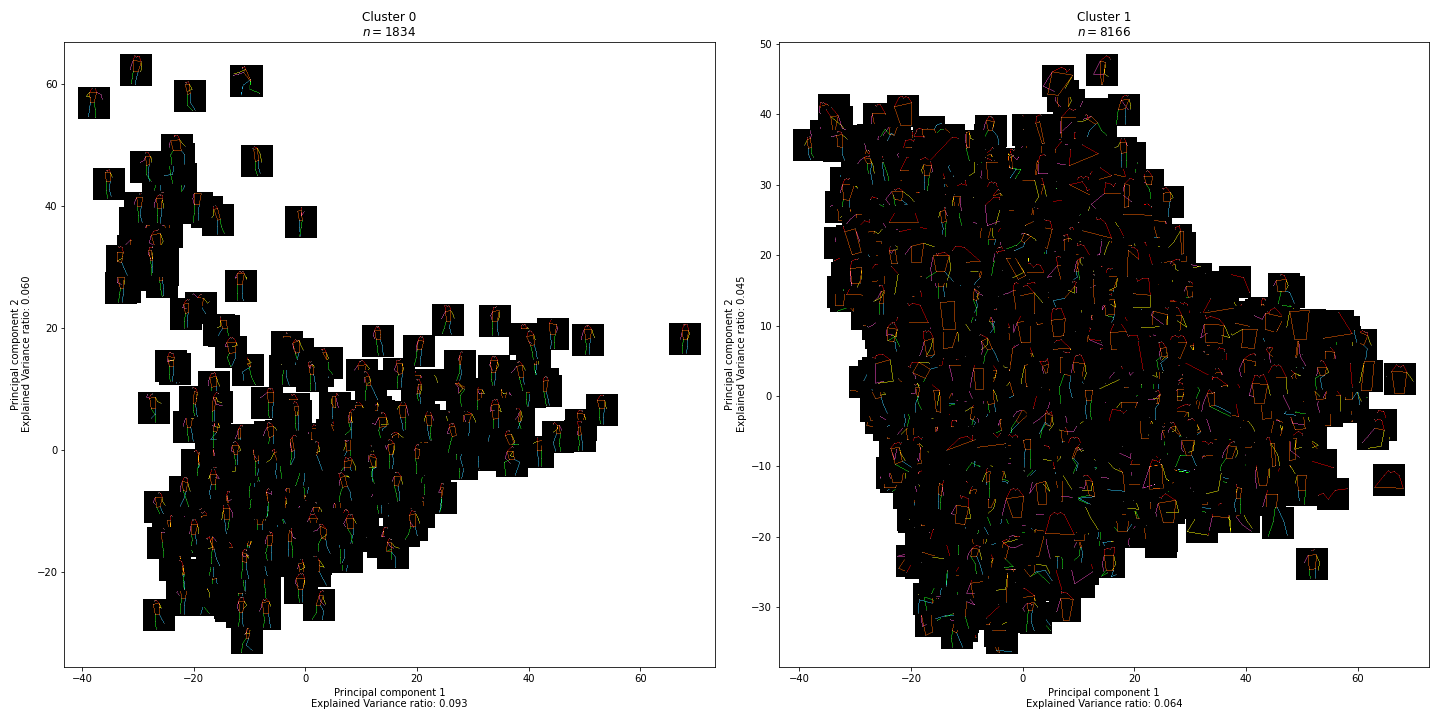
\includegraphics[width = \textwidth]{entities/cluster_all_skeletons.png}
    \caption{The resulting clusters of running a $K$-Means model with $K = 2$ on the latent space consisting of $10.000$ random training samples}
    \label{fig:clusters_all_skeletons}
\end{figure}
\\
The results of running the $K$-Means model with $K = 2$ has been visualized in Figure \ref{fig:clusters_all_skeletons}. The $K$-Means model were ran on the latent space in all of the $4.096$ dimensions and only each cluster were projected down to $2$ dimensions for the purpose of visualization. By looking at Figure \ref{fig:clusters_all_skeletons} we can see how the two clusters has different content: where Cluster $0$ focuses more on almost fully-annotated samples, Cluster $1$ focuses more on samples that have a lot of keypoints missing. This is also easy to see if we look at the ground truth heatmaps of the samples closest to the centroids of the two clusters, as visualized in Figure \ref{fig:centroids_all}. By doing so we can see, that the ground truth heatmap of the closest sample to the centroid of Cluster $0$ almost has all of its joints annotated, whereas the ground truth heatmap of the closest sample to the centroid of Cluster $1$ only consists of $2$ keypoints.
\\
\begin{figure}[htbp]
    \centering
    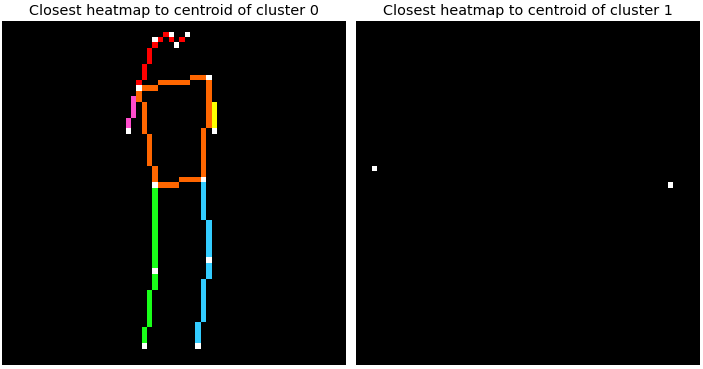
\includegraphics[height = 4 cm]{entities/centroids_all_skeletons.png}
    \caption{Closest points to the centroids of the two clusters from running $K$-Means on the latent space consisting of $10.000$ random training samples}
    \label{fig:centroids_all}
\end{figure}
\\
Although there are differences in the two clusters in Figure \ref{fig:clusters_all_skeletons}, there are still quite a lot of missclassified samples. To overcome this problem we remove all of the not fully-annotated samples and instead use all of the $7.017$ fully-annotated samples of the training set, again fed through the network and outputted by the third residual module in the bottleneck. By doing so we get the Silhouette scores visualized in Figure \ref{fig:silhouette_full}, where we again clearly see, that $K = 2$ is the optimal value of $K$.
\\
\\
The two clusters, resulted by only using fully-annotated samples, have been visualized in Figure \ref{fig:clusters_full_skeletons} and the corresponding closest ground truth heatmaps for the samples closest to the centroids have been visualized in Figure \ref{fig:centroids_full}. Like before, the $K$-Means model were ran on the data in full dimension to create the two clusters, which then were projected down to $2$ dimensions using PCA for the purpose of visualization. By looking at the figure we clearly see how the content of Cluster $0$ contains samples that are stationary, whereas the samples of Cluster $1$ carry a lot more movement. This is also the case for the ground truth heatmaps of the samples closest to the centroids, visualized in Figure \ref{fig:centroids_full}, as we can see, that the heatmap for Cluster $0$ is more straighten, whereas the heatmapf for Cluster $1$ is more bent and looks like it is in more movement. The two clusters does have a lot less missclassifications, than it was the case with the two clusters in Figure \ref{fig:clusters_all_skeletons}. The missclassifications could explain the not-optimal performance of the model as this could mean, that the network has not fully learned the differences between certain positions and where the positions should be placed in the latent space.
\begin{figure}[htbp]
    \centering
    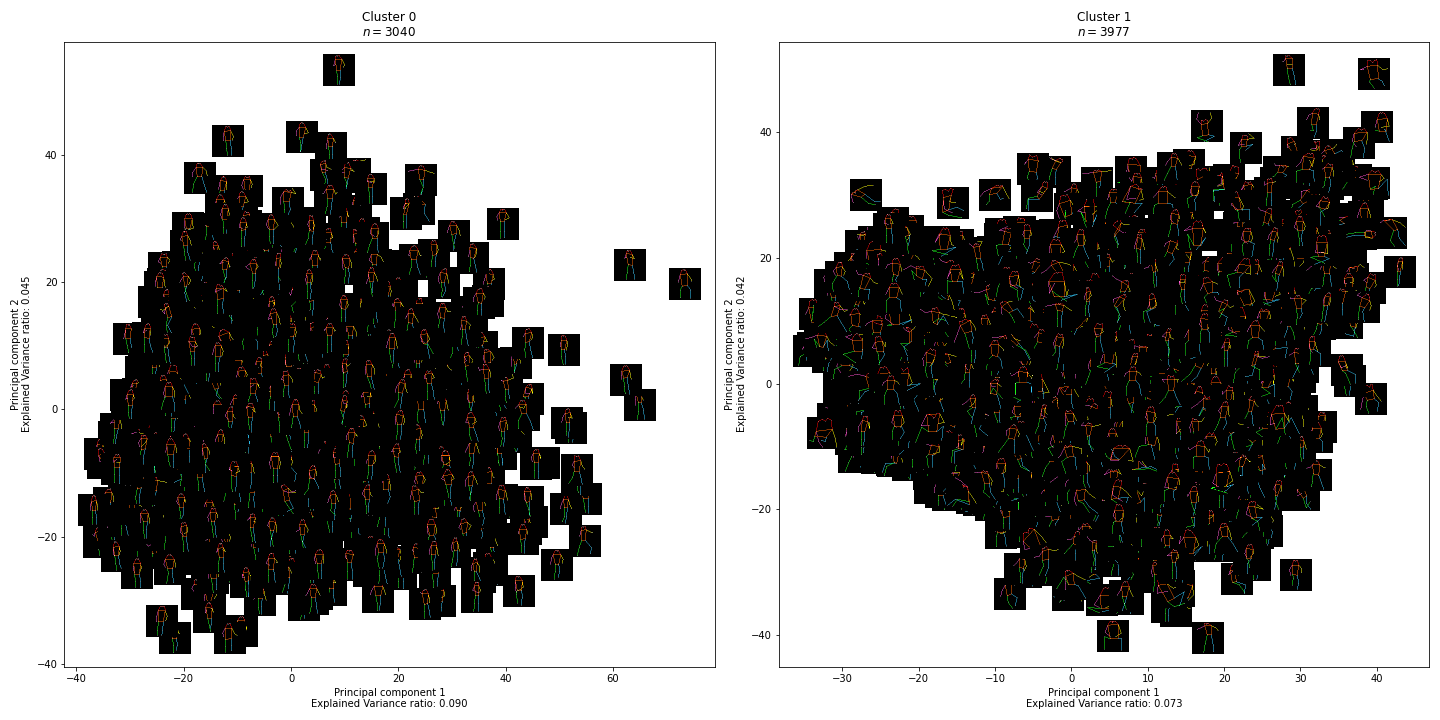
\includegraphics[width = \textwidth]{entities/cluster_full_skeletons.png}
    \caption{The resulting clusters of running a $K$-Means model with $K = 2$ on the latent space consisting of $7.017$ fully-annotated training samples}
    \label{fig:clusters_full_skeletons}
\end{figure}
\begin{figure}[b]
    \centering
    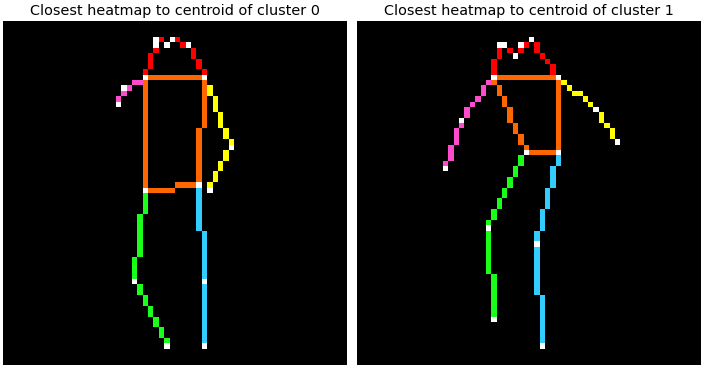
\includegraphics[height = 4 cm]{entities/centroids_full_skeletons.png}
    \caption{Closest points to the centroids of the two clusters from running $K$-Means on the latent space consisting of $7.017$ fully-annotated training samples}
    \label{fig:centroids_full}
\end{figure}
\\
\\
All in all we have learned, that model, during training, has learned to distinguish between almost fully-annotated people and not fully-annotated people, as well as learned to distinguish between stationary people and people with a lot of motion. However, the distinguishments are not perfect, as there are some missclassifications, hinting towards the inaccuracies of the model.

\end{document}